%% This file is a leaflet advertising our MD380 patches, to be
%% tri-folded and distributed at hamfests.  Its margins are wide
%% enough that it should print on either US/Letter or A4 without
%% trouble.

%% STATUS:

%% Most of text is in place.  Additions should aim to include pictures
%% of the more photogenic features (users database).  Photos should be
%% high-contrast, so that they print well in either color or B&W.


\documentclass[
%%notumble,
%%nofoldmark,
%%dvipdfm,
%%portrait,
%%titlepage,
%%nocombine,
%%a3paper,
%%debug,
%%nospecialtricks,
%%draft,
]{leaflet}


\renewcommand*\foldmarkrule{.3mm}
\renewcommand*\foldmarklength{5mm}

\usepackage[T1]{fontenc}
\usepackage{textcomp}
\usepackage{mathptmx}
\usepackage[scaled=0.9]{helvet}
\makeatletter
\def\ptmTeX{T\kern-.1667em\lower.5ex\hbox{E}\kern-.075emX\@}
\DeclareRobustCommand{\ptmLaTeX}{L\kern-.3em
        {\setbox0\hbox{T}%
         %\vb@xt@ % :-)
         \vbox to\ht0{\hbox{%
                            \csname S@\f@size\endcsname
                            \fontsize\sf@size\z@
                            \math@fontsfalse\selectfont
                            A}%
                      \vss}%
        }%
        \kern-.12em
        \ptmTeX}
\makeatother
\let\TeX=\ptmTeX
\let\LaTeX=\ptmLaTeX
\usepackage{shortvrb}
\MakeShortVerb{\|}
\usepackage{url}
\usepackage{graphicx}
\usepackage[dvipsnames,usenames]{color}
\definecolor{LIGHTGRAY}{gray}{.9}

%%%%\renewcommand{\descfont}{\normalfont}
\newcommand\Lpack[1]{\textsf{#1}}
\newcommand\Lclass[1]{\textsf{#1}}
\newcommand\Lopt[1]{\texttt{#1}}
\newcommand\Lprog[1]{\textit{#1}}

\newcommand*\defaultmarker{\textsuperscript\textasteriskcentered}

\title{Patched Firmware for the\\
Tytera MD380!}
\author{
  KK4VCZ, DD4CR, DF8AV, and Friends}
\date{\today}

\CutLine*{1}% Dotted line without scissors
\CutLine{6}%  Dotted line with scissors

%% \AddToBackground{5}{%  Background of a small page
%%   \put(0,0){\textcolor{Cerulean}{\rule{\paperwidth}{\paperheight}}}}

%% \AddToBackground*{2}{% Background of a large page
%%   \put(\LenToUnit{.5\paperwidth},\LenToUnit{.5\paperheight}){%
%%     \makebox(0,0)[c]{%
%%       \resizebox{.9\paperwidth}{!}{\rotatebox{35.26}{%
%%         \textsf{\textbf{\textcolor{LIGHTGRAY}{BACKGROUND}}}}}}}}

\begin{document}

\maketitle
\thispagestyle{empty}

%%\LARGE

%%\tableofcontents


\noindent
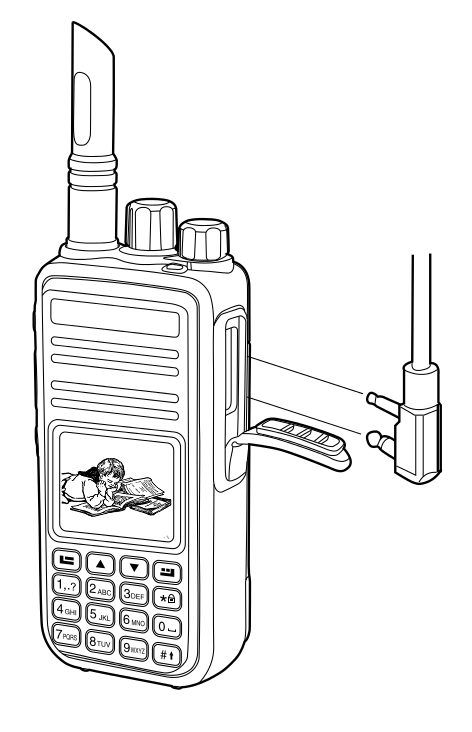
\includegraphics[width=\columnwidth]{figures/md380}


\section{Overview}

The Tytera MD380, also sold under a variety of other brand names, is a
handy-talky for the 2m or 70cm bands in both traditional FM and the
Digital Mobile Radio (DMR) protocol.  Conveniently, it has far better
build quality than a Baofeng and a far lower price than a Motorola.

We've spent the past few months reverse engineering this radio, then
the firmware to add clever new features.  Now that the code is
stabilizing, we'd like to invite you to play along, either by running
our patched firmware or by helping to write it!

\section{Software}

Our patched firmware is developed for the UHF model of the Tytera
MD380, which is also sold as the Retevis RT3.  Most features also
work on the VHF model, which contains a smaller SPI Flash chip.

Our Software Development Kit requires a recent version of Linux with
an {\tt arm-\-none-\-eabi-\-gcc} cross compiler and Python 2.7.  Most
of our patches are written in C, with very little assembly only when
necessary, so skilled programmers can begin adding their own features
without much trouble.

For portable use, we are building an Android application that can
flash the patched firmware through USB OTG.  Like our SDK, the code to
this application is open source.

\section{Features}

Our patched firmware offers a number of nifty new features.

\begin{itemize}

\item
A complete copy of the DMR MARC database can be stored in SPI Flash,
allowing your radio to show the name, callsign, and location of a
distant QSO.

\item
An optional promiscuous mode allows you to hear all talkgroups, even
those that you are not listed in your codeplug.  The talkgroup numbers
are displayed on your radio's screen, so that you know to program
them in later.

\item
A replacement font makes the screen more pleasant to read.

\item
USB logging allows an attached Linux computer to record calls, text
messages, and digital audio.

\item
New menu items allow for on-device programming, such as changes to
your DMR LLID number, without the need to find a laptop computer
and transfer codeplugs.

\end{itemize}

\section{}



\section{Join our gang!}

Source code to our firmware patches and the a suite of Python command-line
tools is available online.
\\{\tt http://github.com/travisgoodspeed/md380tools/}

Source code to our Android application is available in a second repository.
\\{\tt http://github.com/travisgoodspeed/MD380Tool/}
\loggingall
\end{document}
\endinput

